\lecture{10}{26. Februar 2025}{Failure Mechanisms, Pt. 2: Fatigue and Creep}

\section{Fatigue}

\begin{definition}[Fatigue]
  \textit{Fatigue} is a form of failure that occurs in materials subjected to cyclic (repeated) stress over an extended period. Even if the peak stress in each cycle is below the yield strength cracks will gradually initiate and propagate until sudden fracture occurs. In this way fatigue is not about one-time overloading but rather a cumulative effect of repeated (often variable) stresses that eventually lead to crack growth and failure.
\end{definition}

The typical mechanism for a fatigue failure like explained above is that sharp edges of cracks or other defects act as stress concentrators and as such relatively small stresses are required to start growing the cracks that amplify the stress the most. When these cracks start growing they will accelerate in growth speed and at some point these cracks reach a critical size where the cross-section of the uncracked metal can no longer sustain the load and sudden fracture occurs. This is the case for the fractured gear on \textbf{\autoref{fig:f10_1}}.
\begin{figure} [ht]
  \centering
  \caption{Gear fractured due to fatigue}
  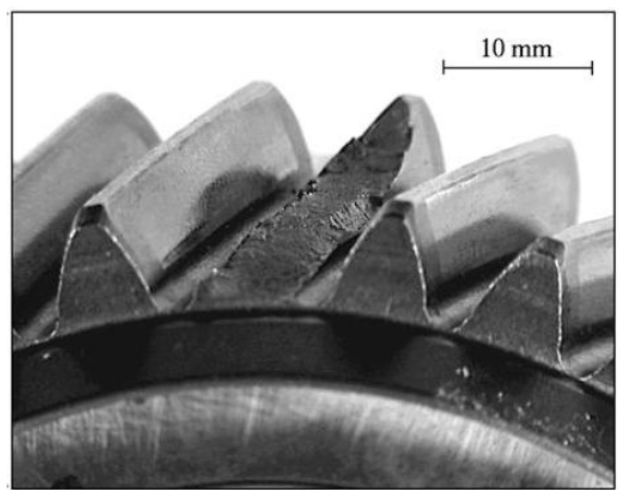
\includegraphics[width=0.5\linewidth]{./figures/f10_1.png}
  \label{fig:f10_1}
\end{figure}


\subsection{Rotating bending test}
To test how a material behaves under cyclic loading (the type of loading that produces fatigue) you often employ a \textit{rotating bending test} where a cylindrical specimen is clamped at both ends and rotated by a motor. The test specimen will also be pulled down by a fixed load. As the specimen rotates different parts of the outer surface of the test specimen will be in compression and tension due to the bending load. This makes one able to standardize the test by fixing the \unit{rpm} and or amount of \unit{rev}'s such that one can compare the fatigue data from the test across different materials.
\begin{figure} [ht]
  \centering
  \caption{Sinusoidal behaviour of fatigue tests}
  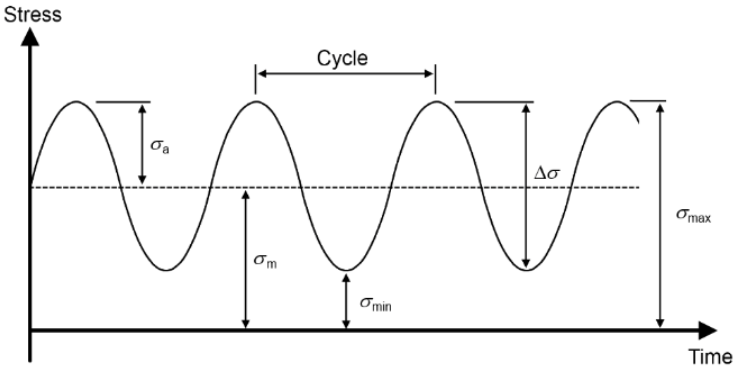
\includegraphics[width=0.5\linewidth]{./figures/f10_2.png}
  \label{fig:f10_2}
\end{figure}
The cycle of such a test is often sinusoidal like shown in \textbf{\autoref{fig:f10_2}}. This also means it is rather easy to calculate the mean stress $\sigma_m$, the stress range $\sigma_r$, the stress amplitude $\sigma_a$ and the stress ratio $R$ as
\begin{align*}
  \sigma_m &= \frac{\sigma_{\mathrm{max} - \sigma_{\mathrm{min}}}}{2} \\
  \sigma_r &= \sigma_{\mathrm{max}} - \sigma_{\mathrm{min}} \\
  \sigma_a &= \frac{\sigma_r}{2} = \frac{\sigma_{\mathrm{max}} - \sigma_{\mathrm{min}}}{2} \\
  R &= \frac{\sigma_{\mathrm{min}}}{\sigma_{\mathrm{max}}}
.\end{align*}


\subsection{S-N Curves}
The data from e.g. a rotating bending test is often plotted on an $S \log N$-plot (an SN curve) as shown on \textbf{\autoref{fig:f10_3}}.
\begin{figure} [ht]
  \centering
  \caption{SN curve for steel and Al}
  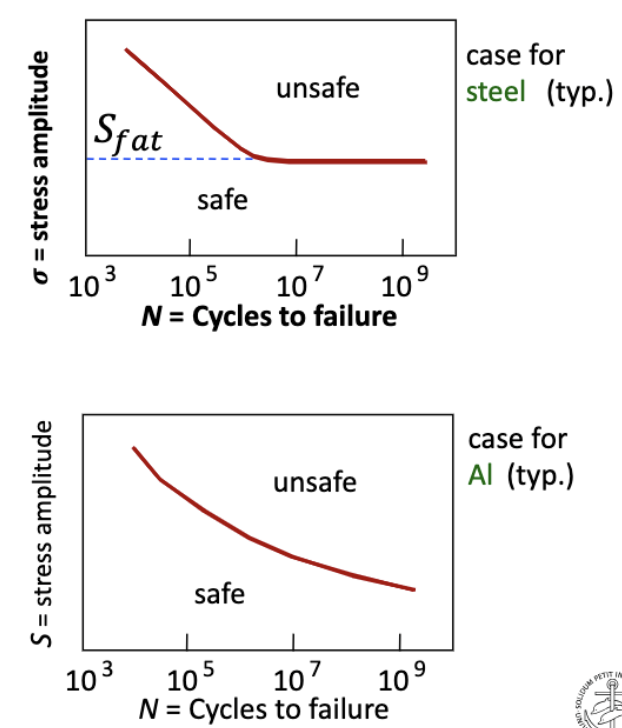
\includegraphics[width=0.25\linewidth]{./figures/f10_3.png}
  \label{fig:f10_3}
\end{figure}
These curves generally look pretty alike for most materials (plus minus some scaling of course), however, there is one point where materials can differ -- namely in terms of the fatigue limit $S_{\mathrm{fat}}$. Not all materials has a fatigue limit (I believe  most do not) but for the materials that do have a fatigue limit fatigue will not accumulate if the applied stress is smaller than the fatigue limit. That is there will be no stress accumulation for $\sigma < S_{\mathrm{fat}}$. This is the case for e.g. steel, whereas aluminum does not have a fatigue limit and it will therefore accumulate fatigue even for very small applied stresses. 

Based on the results from e.g. the rotating bending test a so-called \textit{fatigue limit} $N_f$ can also be calculated. The fatigue limit refers to the total number of stress cycles to cause fatigue failure at a specified stress amplitude.


\subsection{Improving fatigue life}
There are three main techniques to enhance the fatigue life of a component
\begin{itemize}
  \item \textbf{Reducing the magnitude of mean stress:} This is the obvious answer, of course if you want your material to have a longer lifetime you should stress it less.
  \item \textbf{Surface treatments:} Fatigue cracks often initiate at or near the surface, so introducing compressive residual stresses at the surface can help prevent or delay crack initiation. This can be done in many ways. To popular methods work by either shot peening where hard spheres are blasted into the surface of the material which creates compressive stresses due to plastic deformation or by carburizing where $C$-atoms are diffused into the surface layer of the material (creating compressive stresses and hardening the surface).
  \item \textbf{Design changes:} By eliminating sharp corners and other stress concentrators you can also improve the lifespan of your material. 
\end{itemize}

\section{Creep}
Creep is (on top of the name of a hit radio single by Radiohead) a measurement of the deformation (strain) vs. time at a constant stress. Simply put, if you apply a constant stress to something it will deform a bit initially but if you do not remove the stress immediately again the material will start to \textit{creep} and deform (strain) even more even if not changing the applied stress.
\begin{figure} [ht]
  \centering
  \caption{The three stages of creep}
  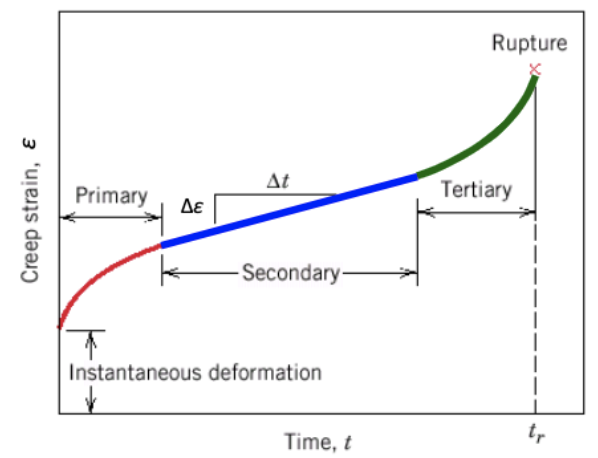
\includegraphics[width=0.5\linewidth]{./figures/f10_4.png}
  \label{fig:f10_4}
\end{figure}

Creep generally happens in three phases
\begin{itemize}
  \item \textbf{Primary creep:} The first phase. Here the creep rate (slop of creep strain vs. time plot) is decreasing with time (creeps a lot at the start and then ``settles in'')
  \item \textbf{Secondary creep:} The second phase. Here the creep is steady-state, meaning the creep rate is increasing linearly with time, i.e. $\frac{\Delta \epsilon}{\Delta t} = \mathrm{const.}$
  \item \textbf{Tertiary creep:} The third phase. Here the creep rate starts accelerating until fracture happens.
\end{itemize}
The above three phases are also shown on \textbf{\autoref{fig:f10_4}}.
The steady state creep rate $\dot{\epsilon}_s$ (secondary phase creep rate) increases with increasing temperature $T$ or stress $\sigma$. Parallel to this is that the rupture lifetime $t_r$ (the amount of time until rupture with a constant stress) decreases with increasing temperature $T$ and stress $\sigma$. This is shown in \textbf{\autoref{fig:f10_5}}.
\begin{figure} [ht]
  \centering
  \caption{The temperature dependence of creep}
  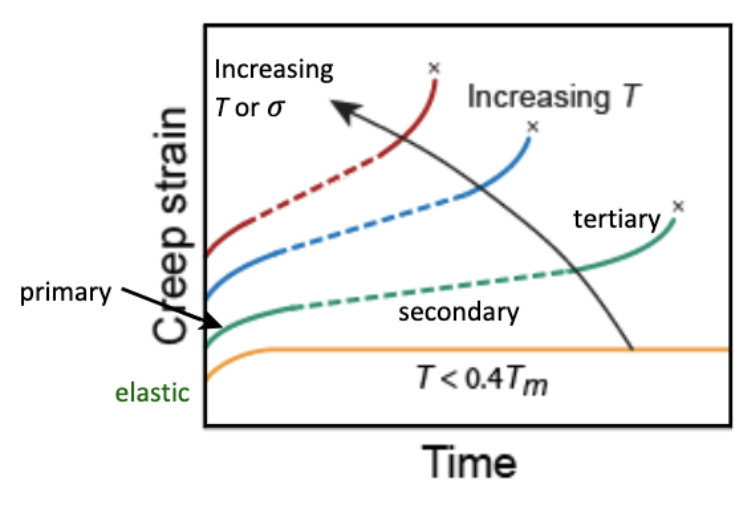
\includegraphics[width=0.5\linewidth]{./figures/f10_5.png}
  \label{fig:f10_5}
\end{figure}

\subsection{Steady-state creep}
The steady-state creep rate $\dot{\epsilon}_s$ (secondary phase creep) is constant for constant temperature $T$ and stress $\sigma$. The steady-state creep rate $\dot{\epsilon}_s$ can be calculated as
\[ 
\dot{\epsilon}_s = K_2 \sigma^{n} e^{-\frac{Q_c}{RT}}
.\]
Where $K_2$ is a material constant, $Q_c$ is the activation energy for creep, $R$ is the universal gas constant and the stress exponent $n$ is a material parameter. The equation can also be written as
\[ 
\dot{\epsilon}_s = K_1 \sigma^{n}
.\]
Where $K_1$ and $n$ are material parameters.


\subsection{Creep life time}
The time to rupture $t_r$ is a measurement of the amount of time a specimen can handle a given (constant) load before rupturing. It is difficult to gather creep data for a prolonged time (e.g. years) and instead you extrapolate from data collected for a shorter time at higher $T$ using the Larson-Miller parameter $m$, defined as
\[ 
T \left( C + \log t_r \right) = m
.\]
Where $T$ is the temperature, $C$ is a constant (normally $\approx20$, $t_r$ is the time to rupture and the Larson-Miller parameter $m$ is a function of the applied stress. An example of how this can be used is shown in \textbf{\autoref{fig:f10_6}}.
\begin{figure} [ht]
  \centering
  \caption{Example of how to calculate the creep life time using the Larson-Miller parameter}
  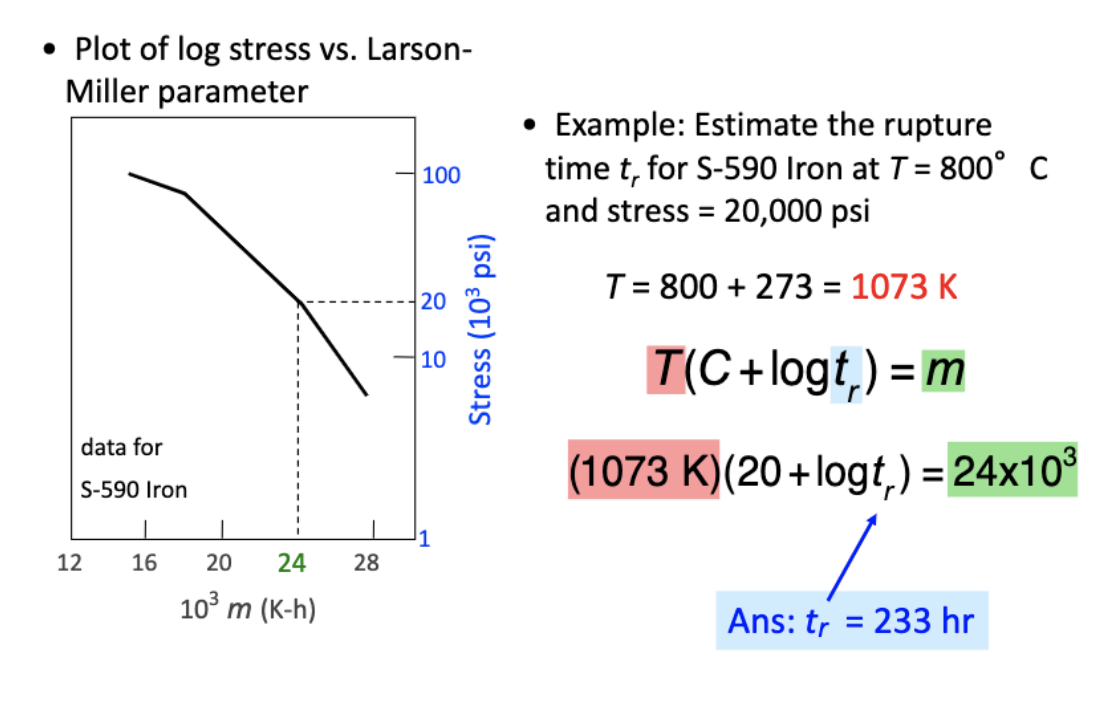
\includegraphics[width=0.5\linewidth]{./figures/f10_6.png}
  \label{fig:f10_6}
\end{figure}
